\chapter{Admission processes in BPMN 2.0}\label{app:jbpm}

	\section{Bachelor's main process}	

	\begin{figure}[h]
		\label{fig:bpm:2012_bsp_main}
		\centering
		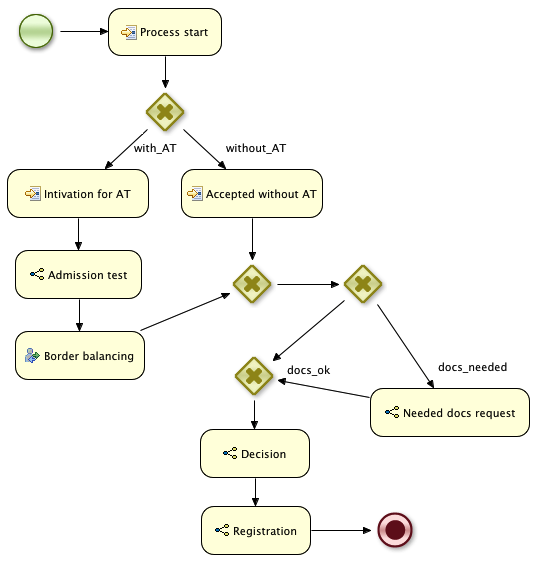
\includegraphics[width=9.4cm]{figures/bpm/2012_bsp_main}
		\caption{Bachelor's admission process for 2012}
	\end{figure}
	
	\newpage
	
	\section{Masters's main process}
	
	\begin{figure}[h]
		\label{fig:bpm:2012_msp_main}
		\centering
		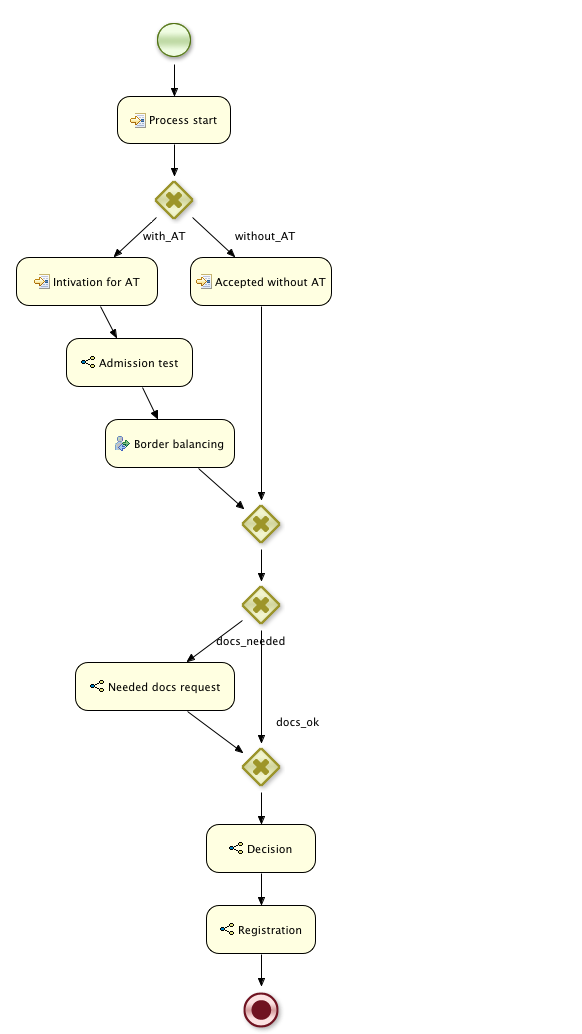
\includegraphics[width=9.4cm]{figures/bpm/2012_msp_main}
		\caption{Master's admission process for 2012}
	\end{figure}
	
	\section{Shared processes}
	
	With closer look at both main processes, it is clear, that they basically share everything. They just differ in
	evaluation, which is parametrized. The rest of the processes is shared across both main ones.

	\begin{figure}[h]
		\label{fig:bpm:2012_registration_E}
		\centering
		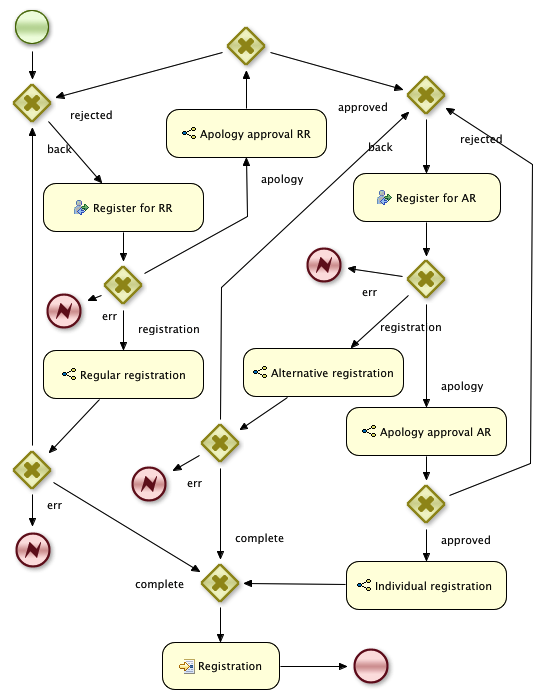
\includegraphics[width=9.4cm]{figures/bpm/2012_registration_E}
		\caption{Registration for 2012}
	\end{figure}

	\begin{figure}[h]
		\label{fig:bpm:2012_admission_test_E}
		\centering
		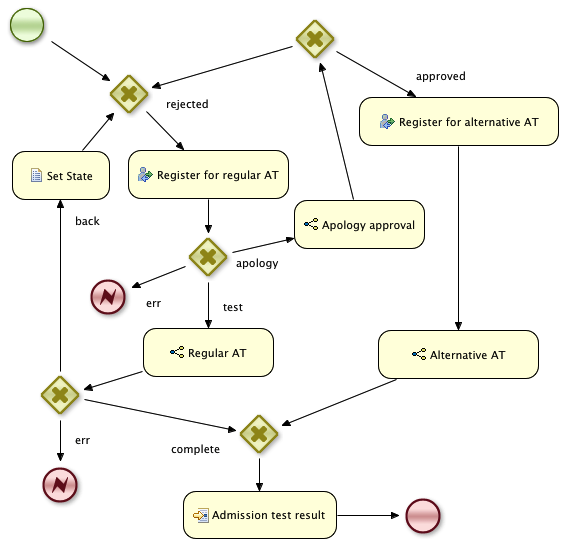
\includegraphics[width=9.4cm]{figures/bpm/2012_admission_test_E}
		\caption{Admission test for 2012}
	\end{figure}

	\begin{figure}[h]
		\label{fig:bpm:2012_decision}
		\centering
		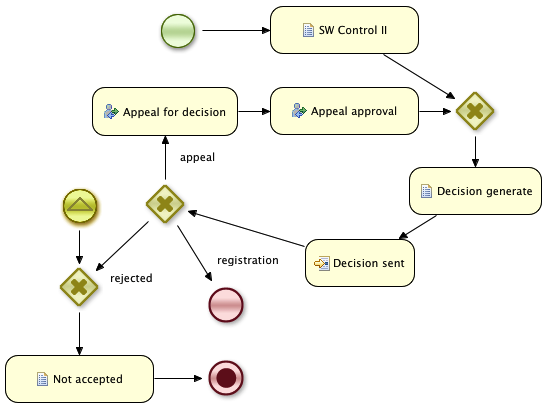
\includegraphics[width=9.4cm]{figures/bpm/2012_decision}
		\caption{Decision for 2012}
	\end{figure}

	\begin{figure}[h]
		\label{fig:bpm:2012_test}
		\centering
		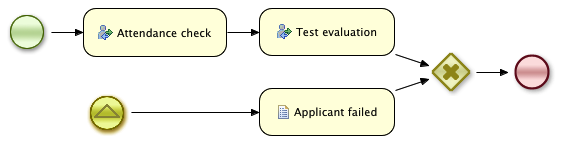
\includegraphics[width=9.4cm]{figures/bpm/2012_test}
		\caption{Test for 2012}
	\end{figure}

	\begin{figure}[h]
		\label{fig:bpm:apology_approval}
		\centering
		
\includegraphics[width=9.4cm]{figures/bpm/apology_approval}
		\caption{Apology approval}
	\end{figure}

	\begin{figure}[h]
		\label{fig:bpm:document_request}
		\centering
		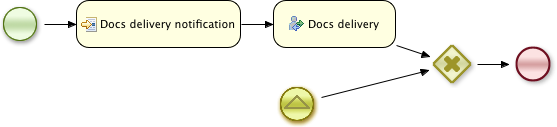
\includegraphics[width=9.4cm]{figures/bpm/document_request}
		\caption{Document request}
	\end{figure}

	\begin{figure}[h]
		\label{fig:bpm:register_to_study}
		\centering
		
\includegraphics[width=9.4cm]{figures/bpm/register_to_study}
		\caption{Register to study}
	\end{figure}
	